% ============================================================
% Report: Question 2 — Traffic Light Controller
% ============================================================

\section{هدف تمرین}
در این سؤال، یک کنترل‌کننده‌ی چراغ راهنمایی برای چهارراهی با دو مسیر شمال–جنوب و شرق–غرب طراحی شده است. پیاده‌سازی به صورت ساختاری انجام شده؛ ماژول اصلی با یک \lr{FSM} سنکرون، دو نمونه از یک ماژول داخلی چراغ را مدیریت می‌کند.

% ============================================================
\section{توضیح معماری}

طراحی از دو ماژول تشکیل شده است:

\begin{itemize}
    \item \code{traffic\_light}: ماژول داخلی و ترکیبی که یک دستور ۲ بیتی دریافت کرده و دقیقاً یکی از سه خروجی \code{green}، \code{yellow} یا \code{red} را فعال می‌کند.
    \item \code{traffic\_light\_controller}: ماژول سطح بالا که شامل \lr{FSM}، شمارنده‌ی \code{timer} و دو نمونه‌ی ساختاری از \code{traffic\_light} برای مسیرهای شمال–جنوب و شرق–غرب می‌باشد.
\end{itemize}

\lr{FSM} دارای ۷ حالت است. از هر حالتی، اگر \code{start=0} شود، \lr{FSM} در سیکل بعدی به \code{STATE\_SAFE} باز می‌گردد. جدول انتقال حالت‌ها به این صورت می‌باشد:

\begin{LTR}
    \begin{table}[H]
        \centering
        \begin{tabular}{|c|c|c|c|c|c|}
            \hline
            \textbf{حالت}             & \textbf{کد} & \textbf{NS} & \textbf{EW} & \textbf{انتقال شرط}                       & \textbf{بعدی حالت} \\
            \hline
            \code{STATE\_SAFE}        & \lr{000}    & قرمز        & قرمز        & \code{start=1}                            & \code{NS\_GREEN}   \\
            \code{STATE\_NS\_GREEN}   & \lr{001}    & سبز         & قرمز        & \lr{timer} $\geq$ \lr{GREEN\_TIME}$-1$    & \code{NS\_YELLOW}  \\
            \code{STATE\_NS\_YELLOW}  & \lr{010}    & زرد         & قرمز        & \lr{timer} $\geq$ \lr{YELLOW\_TIME}$-1$   & \code{ALL\_RED\_1} \\
            \code{STATE\_ALL\_RED\_1} & \lr{011}    & قرمز        & قرمز        & \lr{timer} $\geq$ \lr{ALL\_RED\_TIME}$-1$ & \code{EW\_GREEN}   \\
            \code{STATE\_EW\_GREEN}   & \lr{100}    & قرمز        & سبز         & \lr{timer} $\geq$ \lr{GREEN\_TIME}$-1$    & \code{EW\_YELLOW}  \\
            \code{STATE\_EW\_YELLOW}  & \lr{101}    & قرمز        & زرد         & \lr{timer} $\geq$ \lr{YELLOW\_TIME}$-1$   & \code{ALL\_RED\_2} \\
            \code{STATE\_ALL\_RED\_2} & \lr{110}    & قرمز        & قرمز        & \lr{timer} $\geq$ \lr{ALL\_RED\_TIME}$-1$ & \code{NS\_GREEN}   \\
            \hline
        \end{tabular}
        \caption{جدول انتقال حالت کنترل‌کننده‌ی چهارراه}
    \end{table}
\end{LTR}

اگر \lr{ALL\_RED\_TIME=0} باشد، حالت‌های \code{ALL\_RED\_1} و \code{ALL\_RED\_2} نادیده گرفته می‌شوند تا از ماندن یک سیکل اضافه در آن‌ها جلوگیری شود. دیاگرام \lr{FSM} طراحی‌شده در شکل زیر نشان داده شده است:

\begin{figure}[H]
    \centering
    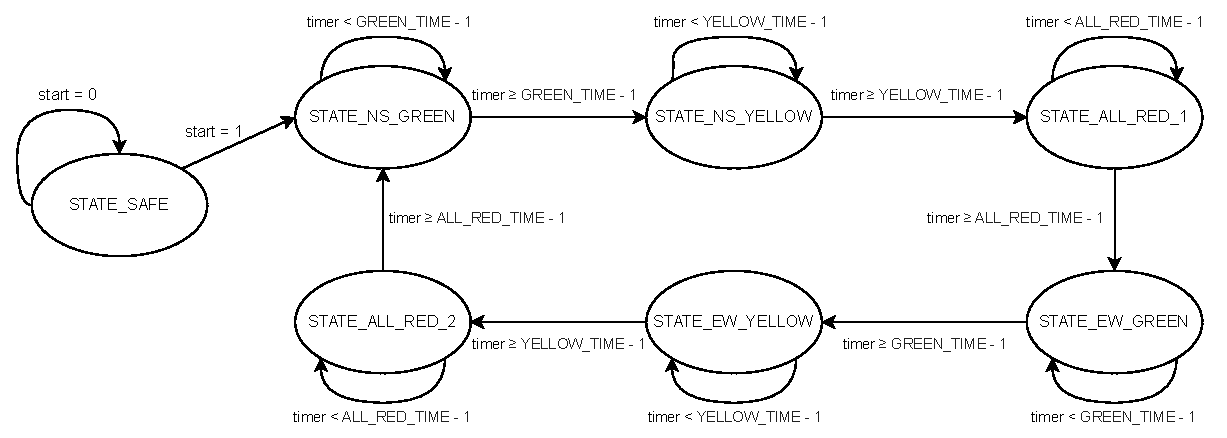
\includegraphics[width=1.0\textwidth]{assets/DSD_HW5_Q2_FSM_diagram.pdf}
    \caption{دیاگرام \lr{FSM} کنترل‌کننده‌ی چهارراه}
\end{figure}

% ============================================================
\section{توضیح کد}

\subsection{ماژول \code{traffic\_light}}
این ماژول یک \lr{decoder} ترکیبی است که دستور ۲ بیتی \code{light\_state} را به سه خروجی \lr{one-hot} تبدیل می‌کند. حالت \lr{2'b11} تعریف نشده؛ \lr{default} آن را نیز قرمز می‌کند تا خروجی همواره معتبر باشد. کد آن به این صورت می‌باشد:

\vspace{0.4cm}
\begin{latin}
    \begin{lstlisting}[language=Verilog]
module traffic_light (
    input wire [1:0] light_state,
    output reg green, output reg yellow, output reg red
);
    always @(*) begin
        case (light_state)
            2'b10: begin green=1; yellow=0; red=0; end // GREEN
            2'b01: begin green=0; yellow=1; red=0; end // YELLOW
            default: begin green=0; yellow=0; red=1; end // RED
        endcase
    end
endmodule
\end{lstlisting}
\end{latin}

\subsection{ماژول \code{traffic\_light\_controller}}
این ماژول از دو بلوک \lr{always} جداگانه ساخته شده که طبق الگوی \lr{two-process FSM} کار می‌کنند.

\textbf{بلوک \lr{Sequential}:} فقط \code{current\_state} و \code{timer} را مدیریت می‌کند. تشخیص تغییر حالت با مقایسه‌ی \code{current\_state} و \code{next\_state} انجام می‌شود؛ در صورت انتقال، \code{timer} ریست می‌شود و در غیر این صورت یک واحد افزایش می‌یابد:

\vspace{0.4cm}
\begin{latin}
    \begin{lstlisting}[language=Verilog]
always @(posedge clk) begin
    if (rst) begin
        current_state <= STATE_SAFE;
        timer         <= 16'd0;
    end else begin
        if (current_state != next_state) begin
            current_state <= next_state;
            timer         <= 16'd0; // reset on every state transition
        end else begin
            timer <= timer + 1'b1;
        end
    end
end
\end{lstlisting}
\end{latin}

\textbf{بلوک \lr{Combinatorial}:} مقدار \code{next\_state} و سیگنال‌های دستور چراغ را محاسبه می‌کند. مقادیر پیش‌فرض در ابتدا ست می‌شوند (نگه‌داشتن حالت و قرمز کردن هر دو مسیر). اگر \code{start=0} باشد، \code{next\_state} مستقیماً به \code{STATE\_SAFE} ست می‌شود؛ در غیر این صورت، \lr{case} بر اساس حالت فعلی اجرا می‌شود:

\vspace{0.4cm}
\begin{latin}
    \begin{lstlisting}[language=Verilog]
always @(*) begin
    next_state     = current_state; // default: hold
    ns_light_state = 2'b00;         // default: RED
    ew_light_state = 2'b00;         // default: RED

    if (!start) begin
        next_state = STATE_SAFE;
    end else begin
        case (current_state)
            STATE_SAFE:
                next_state = STATE_NS_GREEN;

            STATE_NS_GREEN: begin
                ns_light_state = 2'b10; // GREEN
                if (timer >= GREEN_TIME - 1)
                    next_state = STATE_NS_YELLOW;
            end

            STATE_NS_YELLOW: begin
                ns_light_state = 2'b01; // YELLOW
                if (timer >= YELLOW_TIME - 1) begin
                    if (ALL_RED_TIME > 0) next_state = STATE_ALL_RED_1;
                    else                  next_state = STATE_EW_GREEN;
                end
            end

            STATE_ALL_RED_1:
                if (timer >= ALL_RED_TIME - 1) next_state = STATE_EW_GREEN;

            // STATE_EW_GREEN, STATE_EW_YELLOW, STATE_ALL_RED_2
            // follow the same symmetric pattern for the EW direction.

            default: next_state = STATE_SAFE;
        endcase
    end
end
\end{lstlisting}
\end{latin}

\subsection{تست‌بنچ}
\textbf{تسک \code{check\_phase}:}
این تسک بر اساس فاز مورد انتظار (0=\lr{SAFE/ALL\_RED}، 1=\lr{NS\_GREEN}، 2=\lr{NS\_YELLOW}، 3=\lr{EW\_GREEN}، 4=\lr{EW\_YELLOW})، مقادیر صحیح خروجی را از روی مشخصه محاسبه کرده و با خروجی واقعی \lr{DUT} مقایسه می‌کند:

\vspace{0.4cm}
\begin{latin}
    \begin{lstlisting}[language=Verilog]
task check_phase;
    input integer phase;
    reg exp_ns_g, exp_ns_y, exp_ns_r;
    reg exp_ew_g, exp_ew_y, exp_ew_r;
    begin
        test_num = test_num + 1;
        // Reference model: default both directions RED
        exp_ns_g=0; exp_ns_y=0; exp_ns_r=1;
        exp_ew_g=0; exp_ew_y=0; exp_ew_r=1;
        case (phase)
            1: {exp_ns_g,exp_ns_y,exp_ns_r} = 3'b100; // NS GREEN
            2: {exp_ns_g,exp_ns_y,exp_ns_r} = 3'b010; // NS YELLOW
            3: {exp_ew_g,exp_ew_y,exp_ew_r} = 3'b100; // EW GREEN
            4: {exp_ew_g,exp_ew_y,exp_ew_r} = 3'b010; // EW YELLOW
        endcase
        if (ns_green===exp_ns_g && ns_yellow===exp_ns_y && ns_red===exp_ns_r &&
            ew_green===exp_ew_g && ew_yellow===exp_ew_y && ew_red===exp_ew_r)
            // [PASS]
        else
            // [FAIL] with expected vs got
    end
endtask
\end{lstlisting}
\end{latin}

همچنین یک بلوک \code{always @(posedge clk)} در کل شبیه‌سازی اجرا می‌شود که در هر سیکل دو شرط ایمنی را بررسی می‌کند: فعال نشدن همزمان \code{ns\_green} و \code{ew\_green}، و فعال بودن دقیقاً یک چراغ در هر مسیر.

% Replace everything from \textbf{تست‌کیس‌ها:} to end of \subsection{تست‌بنچ}
% with the block below.

\textbf{تست‌کیس‌ها:}

قبل از شروع تست‌های اصلی، \code{rst} اعمال شده و بررسی می‌شود که هر دو مسیر در حالت ایمن باشند:

\begin{latin}
    \begin{lstlisting}[language=Verilog]
// Test 1
apply_reset();
#2;
check_phase(0);
\end{lstlisting}
\end{latin}

\vspace{-0.2cm}
بلافاصله بعد از آزاد شدن \code{rst}، بررسی می‌شود که \code{ns\_red=1} و \code{ew\_red=1} باشند.

تست‌های اصلی به ترتیب زیر هستند:

\vspace{0.8cm}
\begin{latin}
    \begin{lstlisting}[language=Verilog]
// Test 2
repeat(5) @(posedge clk); #2;
check_phase(0);
\end{lstlisting}
\end{latin}

\vspace{-0.2cm}
با \code{start=0}، مدار باید در حالت ایمن بماند. پس از ۵ سیکل بدون \code{start}، هیچ انتقال حالتی نباید رخ داده باشد.

\vspace{0.8cm}
\begin{latin}
    \begin{lstlisting}[language=Verilog]
// Test 3
apply_reset(); start = 1'b1;

@(posedge clk); #2;
check_phase(1);                           // SAFE -> NS_GREEN

repeat(GREEN_TIME) @(posedge clk); #2;
check_phase(2);                           // NS_GREEN -> NS_YELLOW

repeat(YELLOW_TIME) @(posedge clk); #2;
check_phase(0);                           // NS_YELLOW -> ALL_RED

repeat(ALL_RED_TIME) @(posedge clk); #2;
check_phase(3);                           // ALL_RED -> EW_GREEN

repeat(GREEN_TIME) @(posedge clk); #2;
check_phase(4);                           // EW_GREEN -> EW_YELLOW

repeat(YELLOW_TIME) @(posedge clk); #2;
check_phase(0);                           // EW_YELLOW -> ALL_RED

repeat(ALL_RED_TIME) @(posedge clk); #2;
check_phase(1);                           // ALL_RED -> NS_GREEN (repeats)
\end{lstlisting}
\end{latin}

\vspace{-0.2cm}
هر انتقال حالت دقیقاً در لحظه‌ی صحیح بررسی می‌شود. مدت هر حالت مستقیماً از پارامترهای مدار خوانده می‌شود؛ مثلاً \code{repeat(GREEN\_TIME)} سیکل برای ماندن در \code{NS\_GREEN} و سپس \code{check\_phase(2)} برای تأیید ورود به \code{NS\_YELLOW}. در مجموع ۷ چک صریح برای یک سیکل کامل وجود دارد.

\vspace{0.8cm}
\begin{latin}
    \begin{lstlisting}[language=Verilog]
// Test 4
apply_reset(); start = 1'b1;
@(posedge clk);       // posedge 1: SAFE -> NS_GREEN
@(posedge clk); #1;   // posedge 2: NS_GREEN; #1 steps past the edge
start = 1'b0;         // de-assert between posedge 2 and 3 (no race condition)
@(posedge clk); #2;
check_phase(0);
\end{lstlisting}
\end{latin}

\vspace{-0.2cm}
پس از ۲ سیکل در \code{NS\_GREEN}، با \code{start=0}، مدار در سیکل بعدی باید به \code{STATE\_SAFE} برگردد. تأخیر \code{\#1} قبل از \code{start=0} برای جلوگیری از \lr{race condition} با لبه‌ی ساعت است.

\vspace{0.8cm}
\begin{latin}
    \begin{lstlisting}[language=Verilog]
// Test 5
apply_reset(); start = 1'b1;
repeat(2 * 2 * (GREEN_TIME + YELLOW_TIME + ALL_RED_TIME)) @(posedge clk);
\end{lstlisting}
\end{latin}

\vspace{-0.2cm}
مدار برای ۲ سیکل کامل اجرا می‌شود و بلوک \lr{assertion} موازی در هر \lr{posedge} دو شرط ایمنی را چک می‌کند: فعال نشدن همزمان دو چراغ سبز، و فعال بودن دقیقاً یک چراغ در هر مسیر.

\pagebreak

\section{اجرای کد}
نتیجه‌ی اجرای کد به این صورت می‌باشد:

\begin{figure}[H]
    \centering
    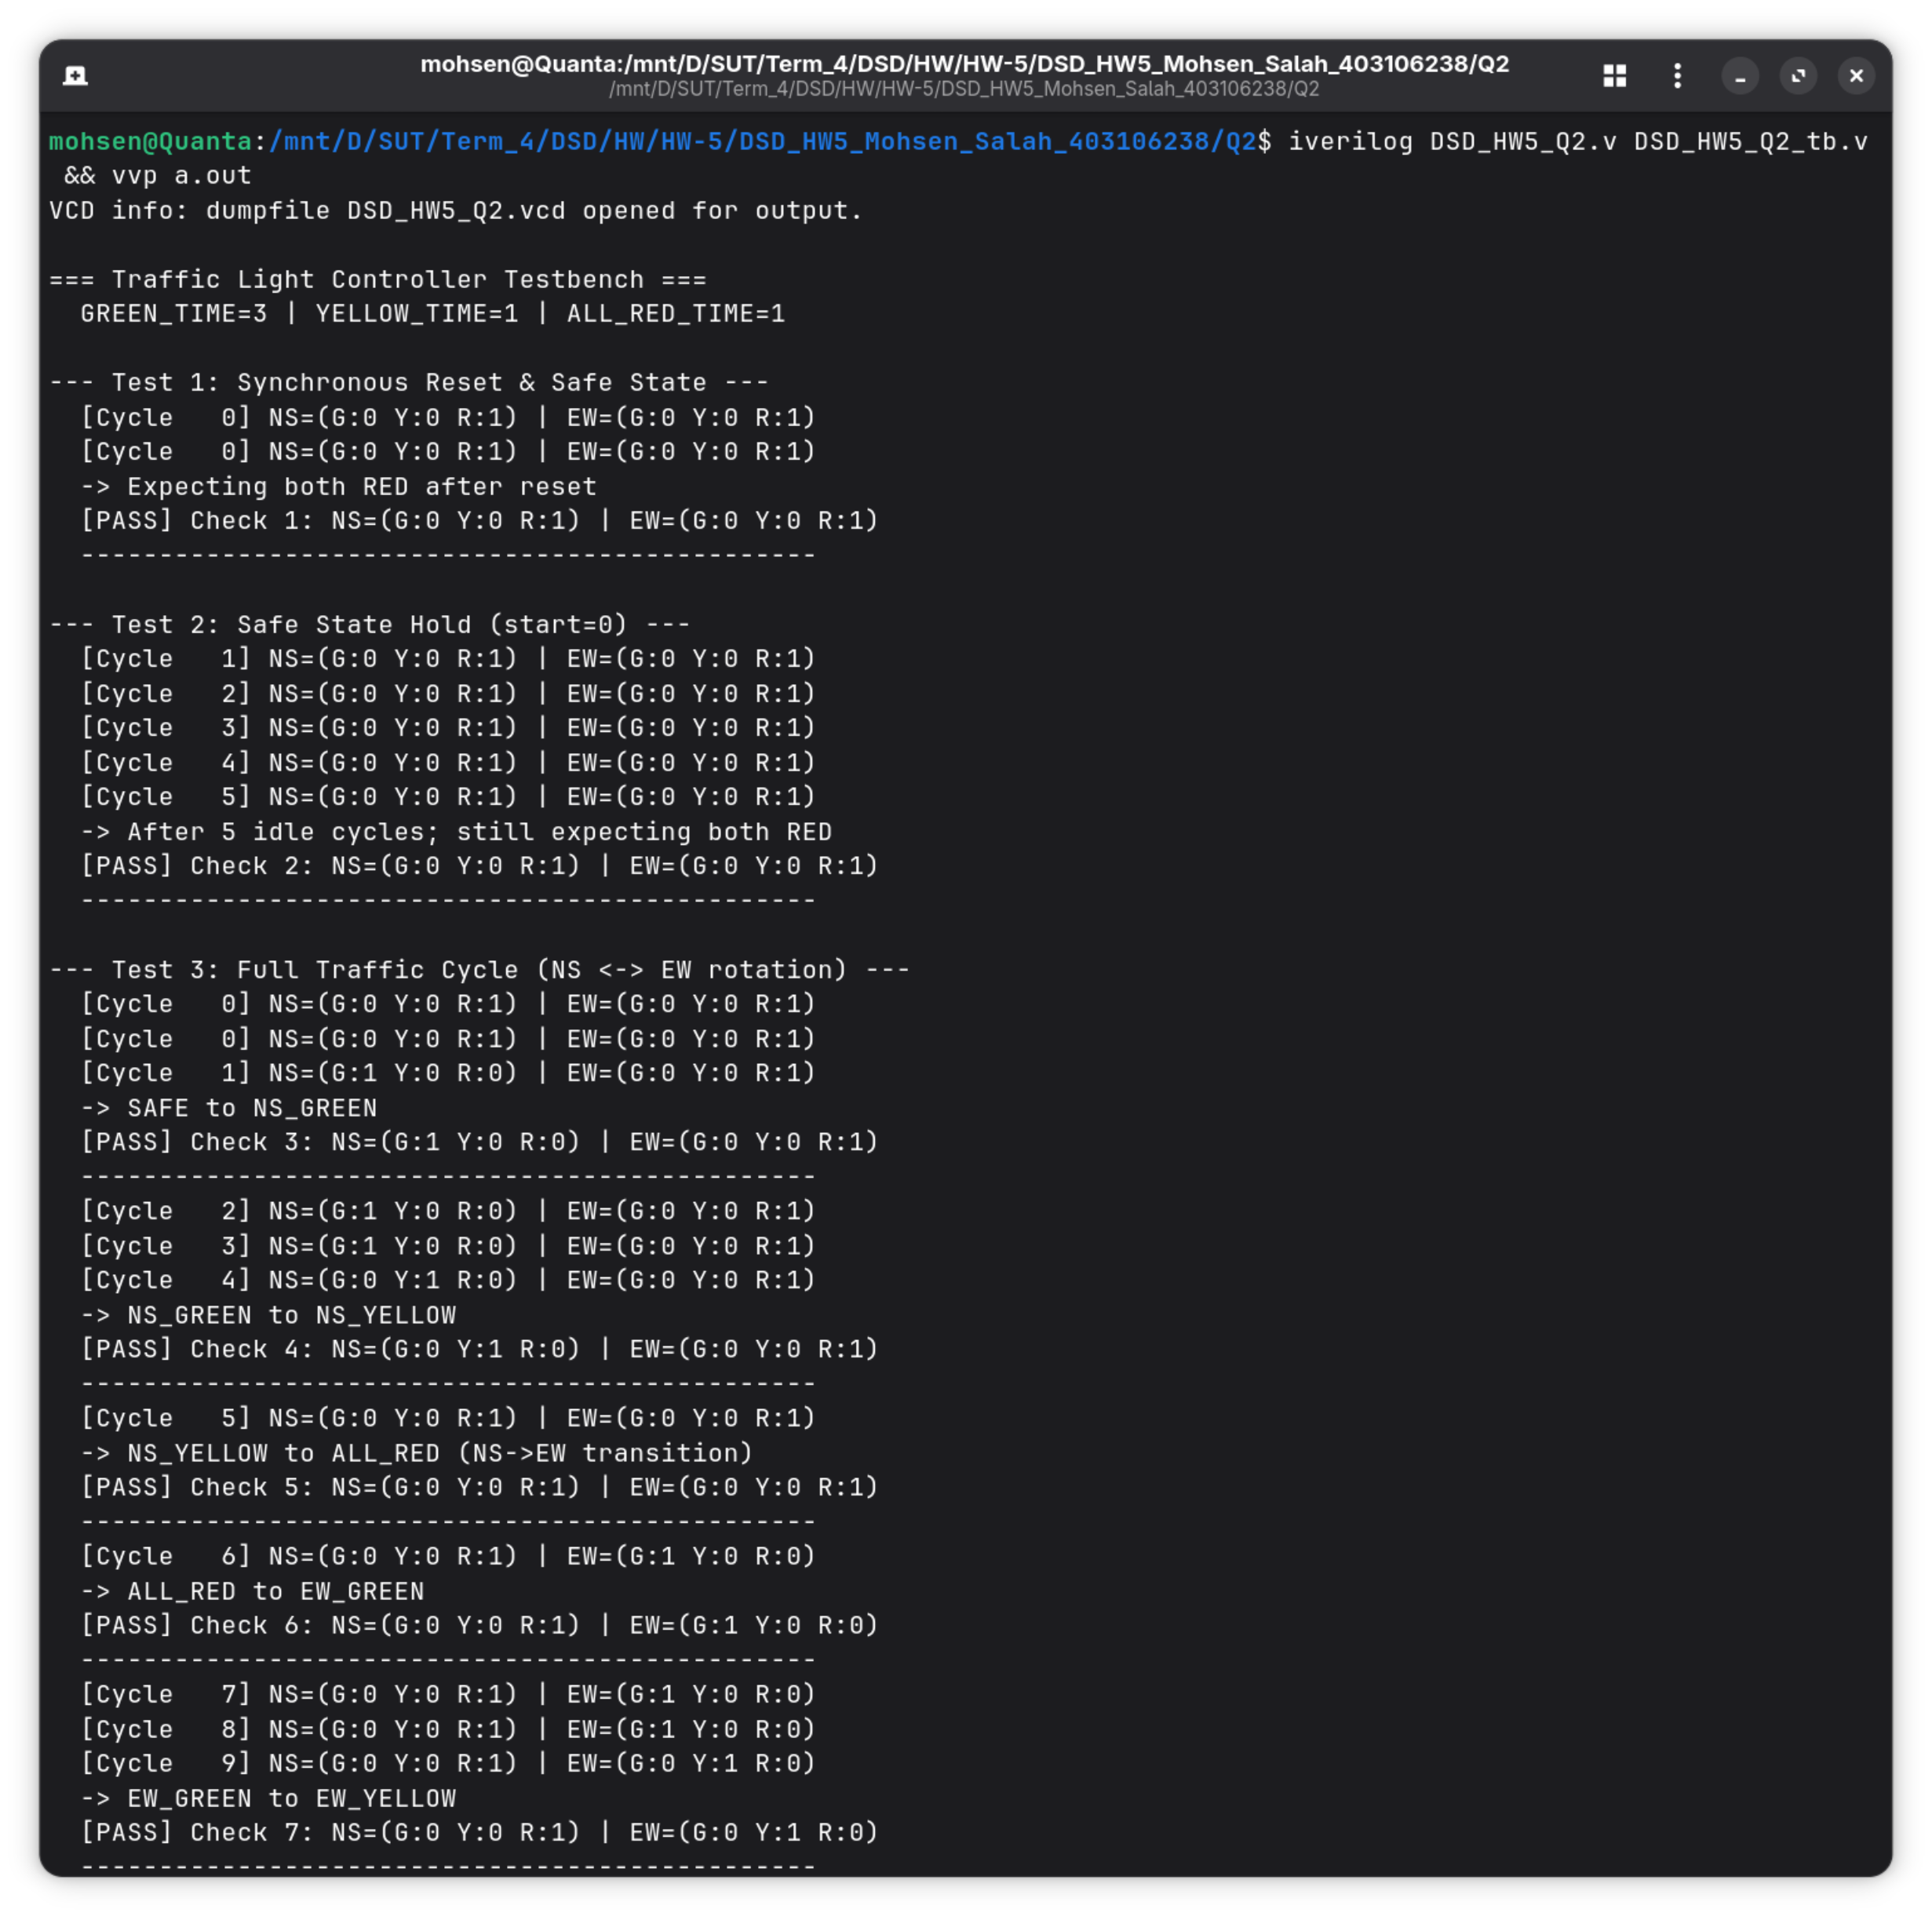
\includegraphics[width=1.0\textwidth]{assets/terminal_1.png}
    \caption{خروجی تست‌بنچ در ترمینال}
\end{figure}

\begin{figure}[H]
    \centering
    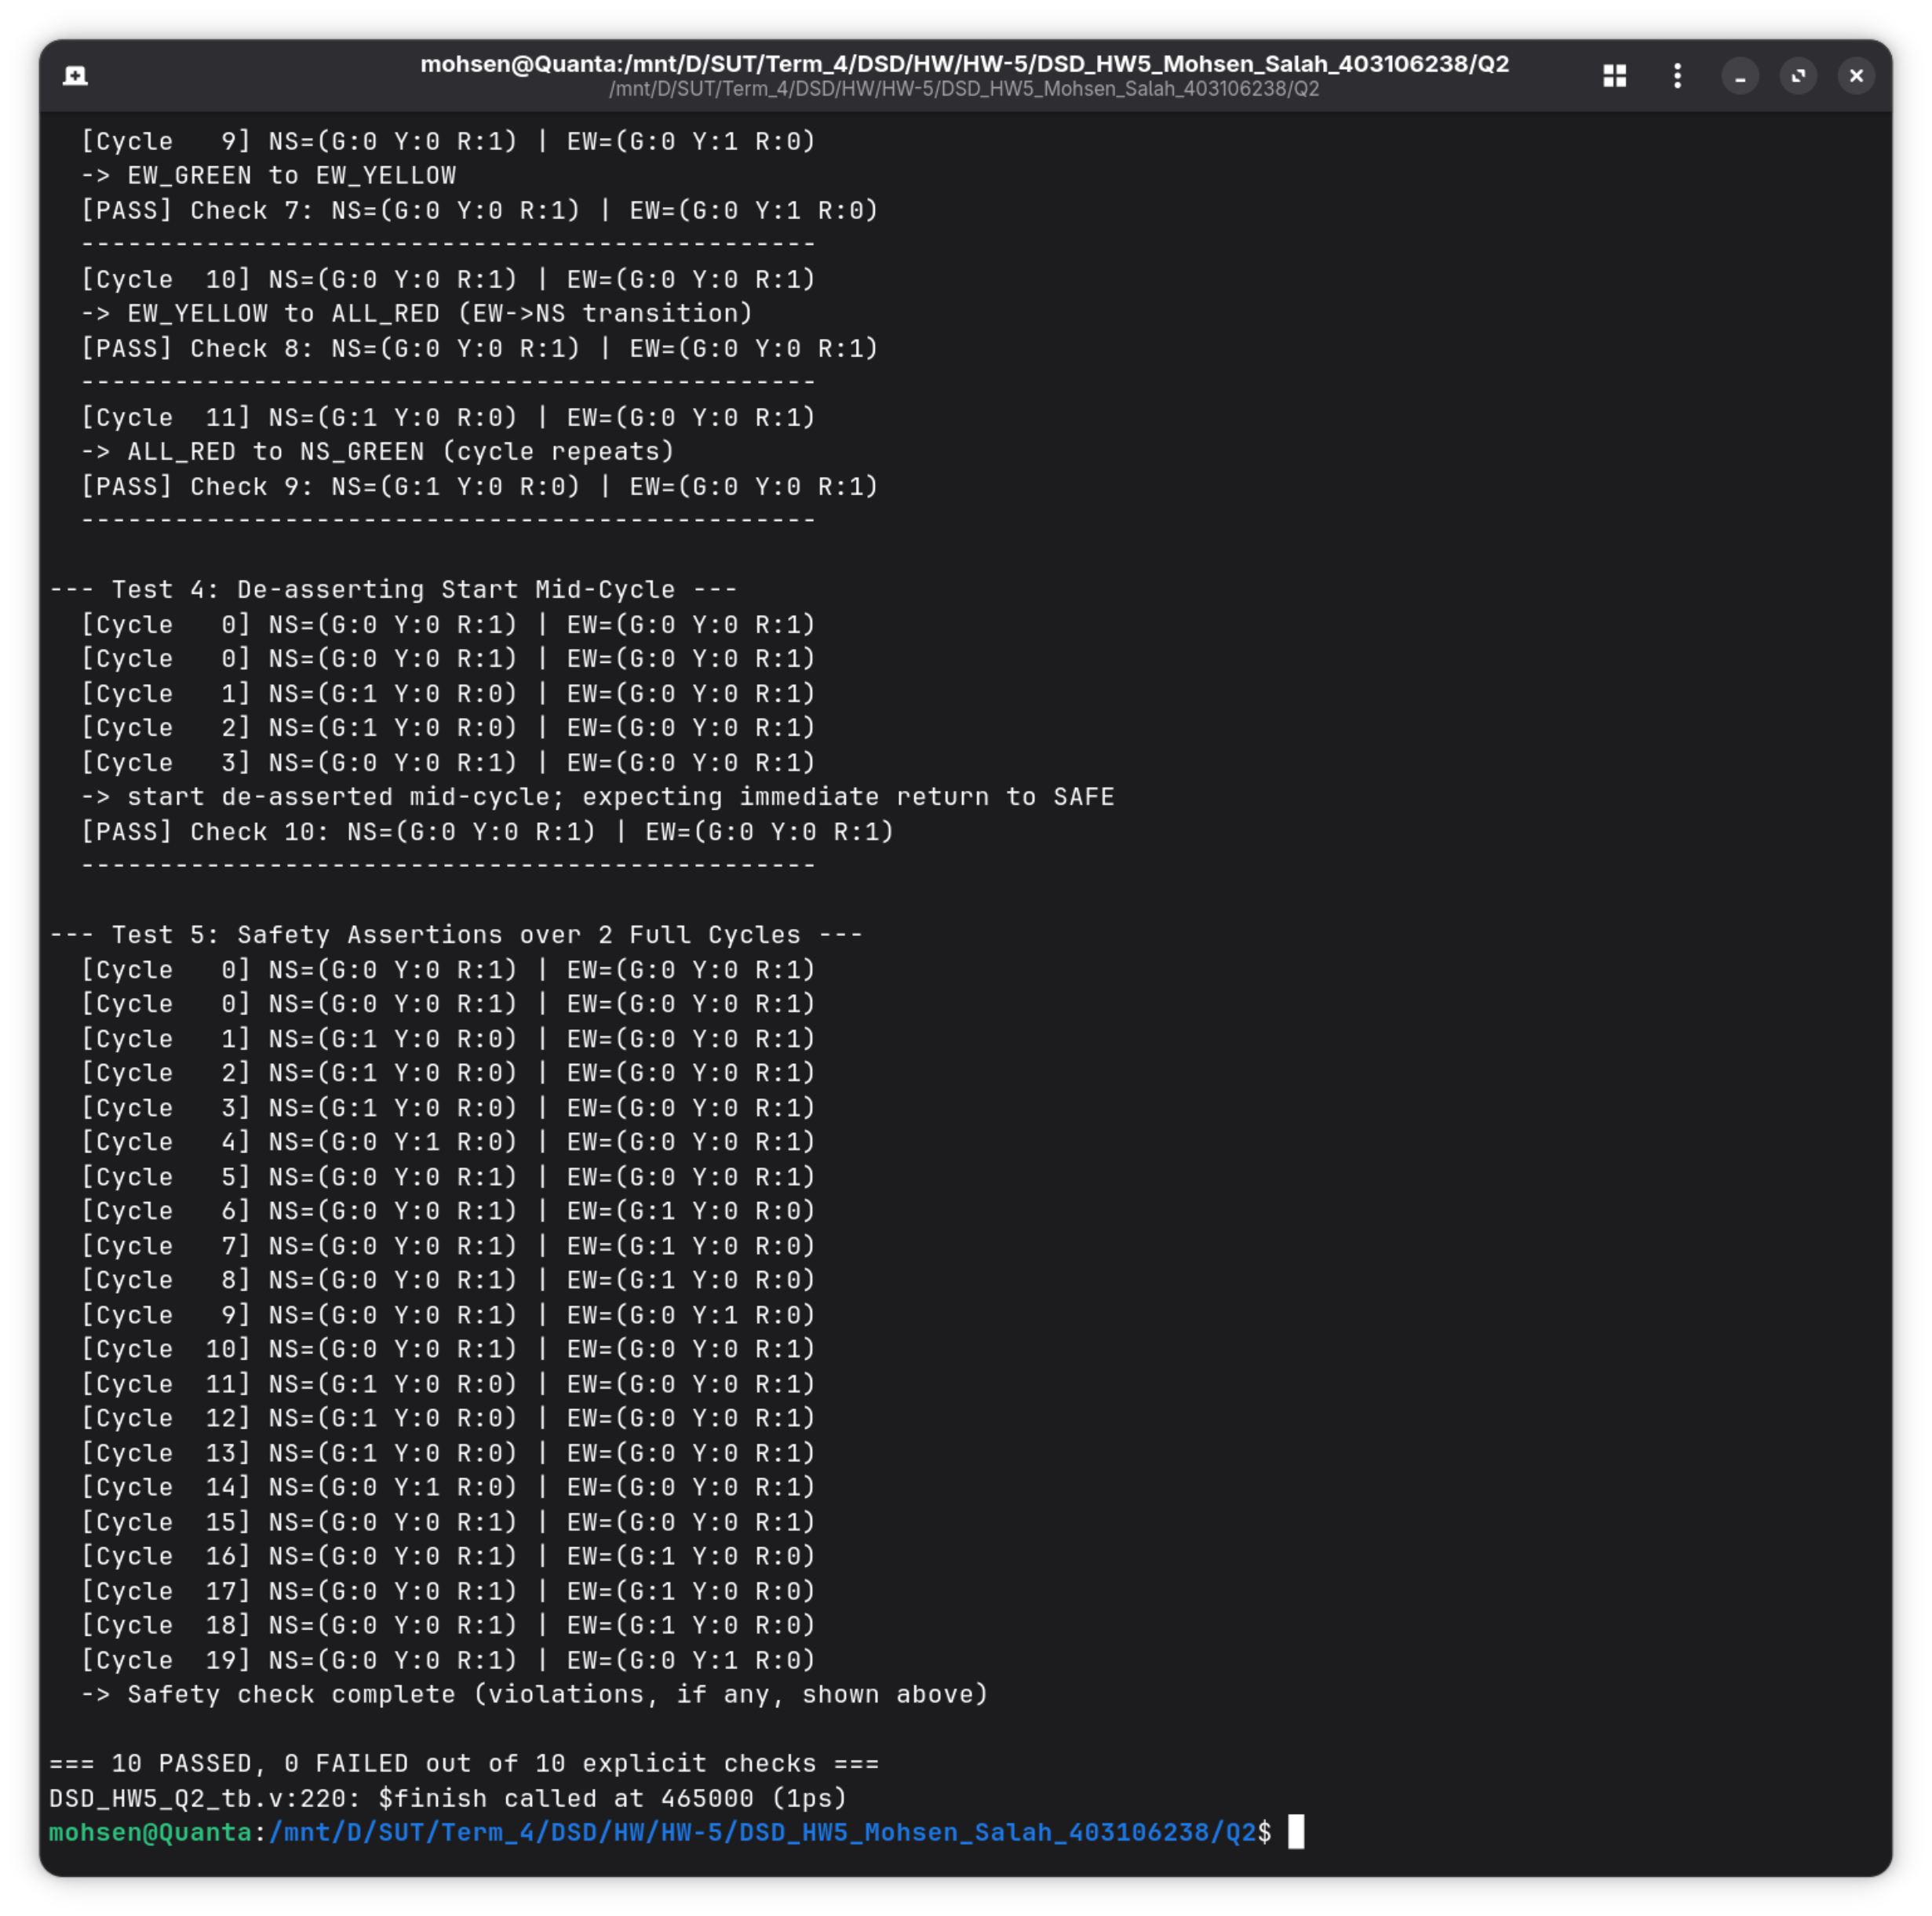
\includegraphics[width=1.0\textwidth]{assets/terminal_2.png}
    \caption{خروجی تست‌بنچ در ترمینال (ادامه)}
\end{figure}

همان طور که مشاهده می‌شود، تمام ۱۰ تست \lr{PASS} شده‌اند.

شکل موج سیگنال‌ها در \lr{GTKWave} نیز به این صورت می‌باشد:

\begin{figure}[H]
    \centering
    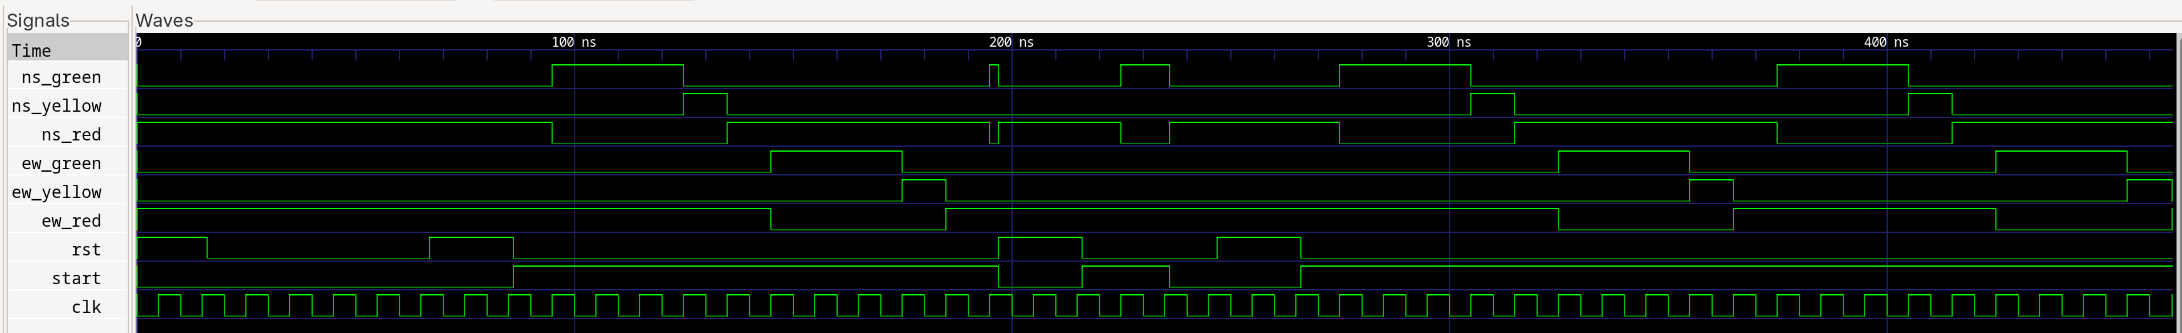
\includegraphics[width=1.0\textwidth]{assets/gtkwave.png}
    \caption{شکل موج سیگنال‌ها در \lr{GTKWave}}
\end{figure}

همان طور که مشاهده می‌شود، ترتیب حالت‌ها و زمان‌بندی چراغ‌ها با جدول معماری طراحی‌شده مطابقت دارد.